\documentclass{fhnwreport/fhnwreport}
\usepackage[ngerman]{babel}
\usepackage[T1]{fontenc}
\usepackage[utf8]{inputenc}
\usepackage[T1]{fontenc}
\usepackage{tikz}
\usepackage{amsmath}
\usetikzlibrary{arrows}
\usepackage{lmodern}   %Type1-Schriftart für nicht-englische Texte
\usepackage{float}

\title{%
  \textsc{Pflichtenheft}\\[2ex]
  \textsc{Technischer Teil}\\[2ex]
  \textsc{FS18 - Pro4E - Team 5}  }
\bibliographystyle{fhnwreport/IEEEtran}  

\begin{document}
\maketitle

\textsc{%
\begin{tabbing}
Auftraggeber: \hspace{4em} \= H. Gysin \\[2ex]
Betreuer:  \>  M. Meier\\[2ex]
\> A. Gertiser \\[2ex]
\> B. Domenghino\\[2ex]
\> P. Schleuniger \\[2ex]
Projektleitung: \> Simon Zoller\\[2ex]
Teammitglieder: \> Severin Hunziker\\[2ex]
\> Mischa Knupfer\\[2ex]
\> Lukas Loosli\\[2ex]
\> Josha Giambonini\\[2ex]
\> Elias von Däniken\\[2ex]
\> Picci\\[2ex]
Studiengang: \> Elektro- und Informationstechnik\\[2ex]
\end{tabbing}
}


\clearpage

\setcounter{tocdepth}{2} 
\tableofcontents
 
\clearpage

%Input Files
%%%%%%%%%%%%%%%%%%%%%%%%%%%%%%%%%%%%%%%%%%%%%%%%%%%%%%%%
\section{Übersicht} 

\subsection{Ausgangslage}
Das Projekt 4 ist für uns Studenten das erste Projekt mit einem externen Auftraggeber. Jana Kalbermatter ist eine Designerin, die auch die Fachhochschule Nordwestschweiz besucht hat. Ihre Bachleor-Arbeit möchte sie nun realiseren.

Sie hat eine Art Audio-Guide für Museen designt, welcher sie Dojo nennt. Ihre Arbeit beinhaltetet das Design des Gehäuses und das dazugehörige Konzept. In ihrem Konzept hat sie die Funktionen des Dojo schon relativ genau definiert, jedoch ist sie offen für neue Ideen. Damit stellt sie die Rahmenbedingungen an das Projekt.

Das Konzept sieht einen Köperschallaktor vor, um die Audio-Files abzuspielen. Eine weitere Eigenheit ist auch der Like Button, mit dem man Ausstellungsstücke "Liken" kann. Diese Likes werden am Ende des Museumsbesuchs zusammengefasst und in einer nicht genauer definierten Form an den Besucher abgegeben. Ansonsten kann der Dojo das was man von einem Audio-Guide erwarten würde.

Die Aufgabe besteht darin in einem ersten Schritt einen funktionierenden Prototypen zu bauen. Dieser soll noch nicht so klein werden, dass er in das ursprüngliche Gehäuse hinein passt. Die Integration soll in einem zweiten Schritt erfolgen. Dies dürfen jedoch nur die Teams machen, die einen genügend guten Prototypen haben.

\begin{figure}[H]
\begin{center}
	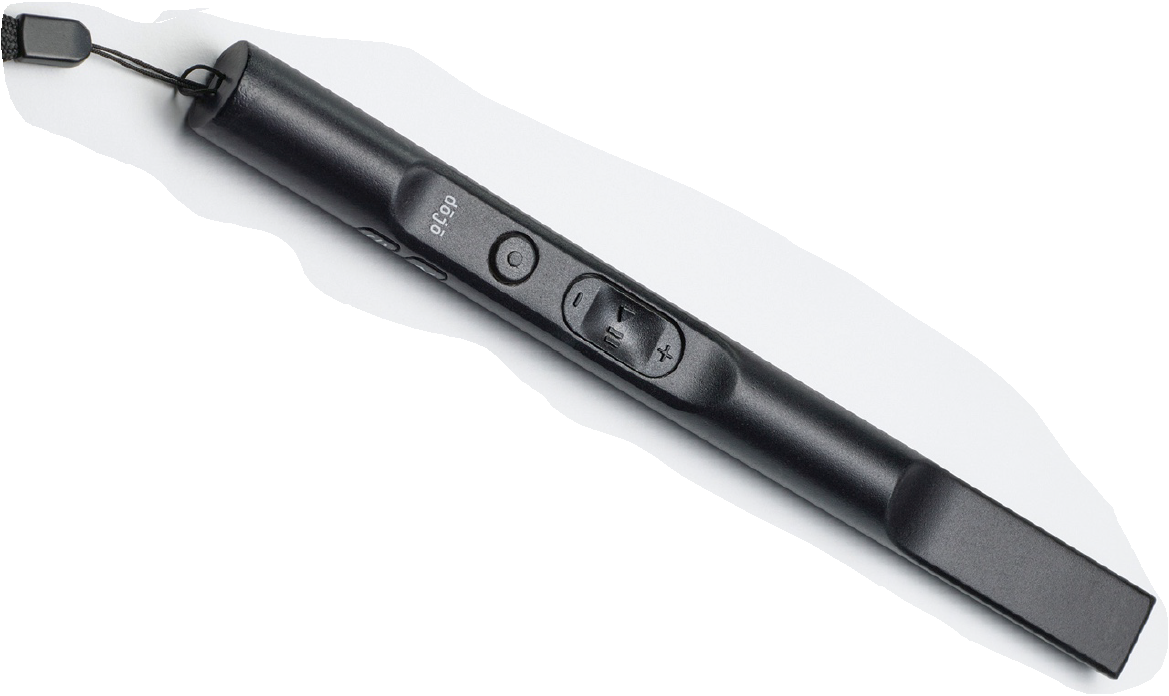
\includegraphics[width=160mm]{data/Ausgangslage_Dojo.png}
	\caption{Konzeptzeichnung des Dojo} %picture caption
	\label{fig:first_layer}
\end{center}
\end{figure}

\pagebreak

\subsection{Projektziele}

\begin{table}[H]
\centering
\begin{tabular}{|c|c|c|}
\hline
\textbf{Nr.:} & \textbf{Muss-Ziele:}                                                  & \textbf{Minimale Anforderungen}                                                                                                                      \\ \hline
1.            & \textbf{Allgemeine}                                                   &                                                                                                                                                      \\ \hline
1.1           & Bedienung                                                             & Die Bedienung des Dojo entspricht dem Lastenheft                                                                                                      \\ \hline
1.2           & Gehäuse                                                               & Am Gehäse wird möglichst wenig verändert                                                                                                            \\ \hline
2.            & \textbf{Audio-Signal}                                                 &                                                                                                                                                      \\ \hline
2.1           & Leistung                                                              & \begin{tabular}[c]{@{}c@{}}Maximale Leistung am\\  Knochenschallaktor 1W/RMS\end{tabular}                                                            \\ \hline
2.2           & Audiodatei                                                            & Audiodatei entsprechend Beacon-ID abspielen.                                                                                                         \\ \hline
2.3           & Aufbereitung                                                          & Filterung (maximale Bandbreite 300Hz-19kHz)                                                                                                          \\ \hline
3.            & \textbf{SD-Karte}                                                     & \begin{tabular}[c]{@{}c@{}}Datentransfer (Daten können gelesen und \\ geschrieben werden)\end{tabular}                                               \\ \hline
4.            & \textbf{Induktives Laden}                                             & die Ladung erfolgt Induktiv                                                                                                                          \\ \hline
5.            & \textbf{Energiespeicher}                                              &                                                                                                                                                      \\ \hline
5.1           & Kapazität                                                             & 500mAh                                                                                                                                               \\ \hline
5.2           & Elektrischer Schutz                                                   & \begin{tabular}[c]{@{}c@{}}Tiefenentladung \& Überladung durch \\ Regelung vermeiden\end{tabular}                                                    \\ \hline
5.3           & Grösse                                                                & 17 x 17 x 55mm                                                                                                                                       \\ \hline
5.4           & Aufladen                                                              & Überladen durch Regelung vermeiden                                                                                                                   \\ \hline
5.5           & Montage                                                               & Montage auf Printplatine                                                                                                                              \\ \hline
6.            & \textbf{Bluetooth}                                                    &                                                                                                                                                      \\ \hline
6.1           & \begin{tabular}[c]{@{}c@{}}Lokalisation \\ Kunstobjekt\end{tabular}   & Erkennung von Beacons auf 3 m Entfernung                                                                                                             \\ \hline
6.2           & \begin{tabular}[c]{@{}c@{}}Identifikation \\ Kunstobjekt\end{tabular} & \begin{tabular}[c]{@{}c@{}}Automatische Auswahl von Beacon mit \\ stärkstem  Signal und Unterscheidung der \\ Beacons mittels Beacon-ID\end{tabular} \\ \hline
              & \textbf{Wunschziele:}                                                 &                                                                                                                                                      \\ \hline
1.            & Daten-Austausch                                                       & \begin{tabular}[c]{@{}c@{}}Bluetooth-Funktionserweiterung um Daten in Dojos\\   Speicher zu laden/löschen\end{tabular}                               \\ \hline
2.            & Lokalisation Dojo                                                     & Sendender Dojo-ID auf Anfrage (via Bluetooth)                                                                                                        \\ \hline
\end{tabular}
\caption{Projektziele}
\label{Projektziele}
\end{table}

\subsection{Lieferobjekte}
\begin{table}[H]
\centering
\begin{tabular}{|l|l|l|l|}
	\hline 
	Objekt & Form & Empfänger & Termin \\ 
	\hline 
	\begin{tabular}[c]{@{}l@{}}Kriterien der Zusammen- \\arbeit (KIS)\end{tabular} & Als PDF per E-Mail & Arbeitgeber /Fachbetreuer & 20.02.18  \\ 
	\hline 
	Pflichtenheft org. Teil & Als PDF per E-Mail & Arbeitgeber /Fachbetreuer & 13.03.18 \\ 
	\hline 
	Pflichtenheft tech. Teil v1 & Als PDF per E-Mail & Arbeitgeber /Fachbetreuer & 13.03.18 \\ 
	\hline 
	Pflichtenfheft tech. Teil  & Als PDF per E-Mail & Arbeitgeber /Fachbetreuer & 27.03.18 \\ 
	\hline 
	Statusbericht 1 & Als PDF per E-Mail & Arbeitgeber /Fachbetreuer & 27.03.18 \\ 
	\hline 
	Zwischenpräsentation & Englisch mündlich & Projektdozenten & 10.04.18 \\ 
	\hline 
	Statusbericht 2 & Als PDF per E-Mail & Arbeitgeber /Fachbetreuer & 28.04.18 \\ 
	\hline 
	Einleitung und Disposition & Als PDF per E-Mail & R.Dubach & 08.05.18 \\ 
	\hline 
	Statusbericht 3 & Als PDF per E-Mail & Arbeitgeber /Fachbetreuer & 15.05.18 \\ 
	\hline 
	Statusbericht 4 & Als PDF per E-Mail & Arbeitgeber /Fachbetreuer & 05.06.18 \\ 
	\hline 
	Schlusspräsentation & Englisch mündlich & Projektdozenten & 12.06.18 \\ 
	\hline
	Fachbericht & gebundenes Heft & Arbeitgeber /Fachbetreuer & 12.06.18\\ 
	\hline
	PMA-Bericht & gebundenes Heft & P.Buchschacher & 12.06.18 \\ 
	\hline 
	Dojo & Print & Arbeitgeber /Fachbetreuer & 12.06.18 \\ 
	\hline
	Projektdaten & USB-Stick & Arbeitgeber /Fachbetreuer & 12.06.18 \\ 
	\hline
\end{tabular} 
\caption{Lieferobjekte}
\label{Lieferobjekte}
\end{table}

\section{Lösungskonzept}
Das Lösungskonzept soll von aussen nach innen definiert werden. Darum werden zuerst die Systemgrenzen definiert. Anschliessend werden die Funktionen beschrieben. Diese werden nachfolgend in Teilsysteme unterteilt. Am Schluss wird noch ein alternativer Ansatz diskutiert, der aber nicht weiterverfolgt wird.

\subsection{Systemgrenzen}
Wie dem nachfolgendem Diagramm entnommen werden kann, wird sich das Projekt auf den Dojo konzentrieren. Alle Systeme die es für das Gesamtsystem Museum braucht, sollen nicht betrachtet werden. Die Schnittstellen werden soweit definiert, dass die Einbindung in ein Gesamtsystem keine Probleme bereiten sollte.

\begin{figure}[H]
\begin{center}
	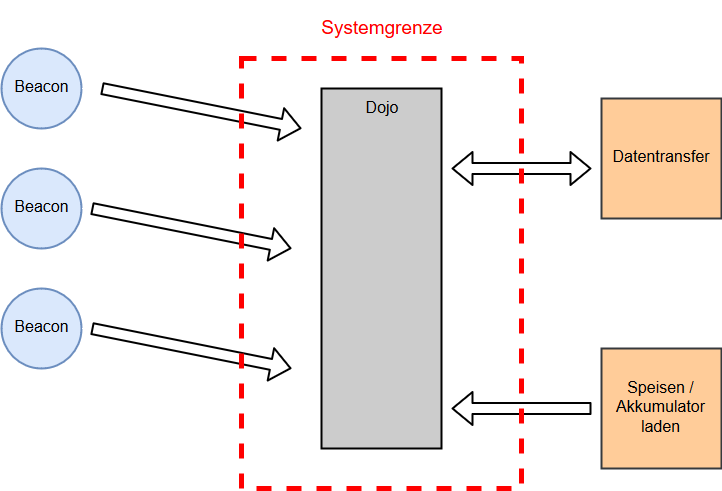
\includegraphics[width=140mm]{data/Loesungskonzept_Systemgrenzen.png}
	\caption{Systemgrenzen des Dojo} %picture caption
	\label{fig:first_layer}
\end{center}
\end{figure}

\subsection{Funktionen}
Die Funktionen sind in zwei Bereiche unterteilt. Einerseits sind die Funktionen für die Museumsbesucher beschrieben, welche nachfolgend als Nutzer bezeichnet werden. Zum anderen die für die Museumsbetreiber relevanten Funktionen. Diese werden nachfolgend als Betreiber bezeichnet.
\subsubsection*{Nutzer}
Der Nutzer geht mit dem Dojo durch das Museum. Sobald die Bluetooth Beacons genug nahe sind, wird dem Nutzer ein Signal gesendet. Dies erfolgt durch Vibration oder mithilfe einer LED. Jetzt soll der Nutzer entscheiden ob er sich das zugehörige Audio-File anhören will. Will er das, kann er den Play-Button betätigen. Die Lautstärke kann über die Buttons justiert werden. Falls das Ausstellungsstück dem Nutzer gefallen hat, kann er die Merken-Taste betätigen. Diese speichert das Ausstellungsstück auf eine Liste im Dojo. Am Ende des Museumsbesuches kann diese Liste ausgewertet werden. Dies fällt aber nicht mehr in die zuvor definierten Systemgrenzen. Wir stellen nur sicher, dass die Liste exportiert werden kann.
\subsubsection*{Betreiber}
Der Betreiber muss den Dojo konfigurieren. Dies erfolgt über eine SD-Karte, welche mit dem Computer beladen wird. Anschliessend wird diese in den Dojo eingeführt. Das Nachladen des Akkumulator erfolgt über eine induktive Ladung. Die nächsten zwei Funktionen sind Wunschziele, die vor allem mit Rücksicht auf die Laufzeit realisiert werden. Den Bluetooth-Reciver könnte man kurzzeitig auf ein Bluetooth Beacon umschalten. Der Betreiber müsste nur noch einen Reciver pro Raum installieren. Damit könnte man die gewünschte HeatMap realisieren. Das zweite wäre die Möglichkeit per Bluetooth einzelne Audiofiles auf den Dojo zu übertragen, um im Falle einer Änderung der Austellung die Liste anzupassen.

\subsection{Teilsysteme}
Das Herzstück des Dojo ist ein NRF52 von Nordic Semiconductor mit integriertem Bluetooth-Stack, welcher wiederum low-Energy fähig ist. Die Daten werden auf einer SD-Karte gespeichert. Der NRF52 wird die Audiodaten an den Verstärker weitergeben, welcher sie über den Körperschallaktor ausgibt. Gespeist wird der Dojo von einem Akku, welcher induktiv geladen wird. Diese Teilsysteme werden in den nachfolgenden Kapiteln noch genauer erläutert.

\begin{figure}[H]
\begin{center}
	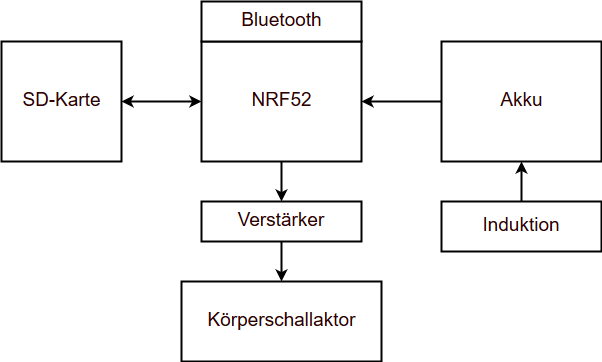
\includegraphics[width=120mm]{data/Loesungskonzept_Teilsysteme.png}
	\caption{Teilsysteme des Dojo} %picture caption
	\label{fig:first_layer}
\end{center}
\end{figure}


\subsection{Alternativer Ansatz}
Im unterstehenden Bild wird der alternative Ansatz gezeigt. Es gibt mehrere Gründe die gegen diesen Ansatz sprechen.
\begin{itemize}
\item Der Mux ist schwierig zu realisieren
\item Die SD-Karte über USB zu beladen ist anspruchsvoll
\item Auf den meisten Bluetooth-Modulen(HM-10) ist ein ähnlicher Chip verbaut wie der NRF52
\item Induktives Laden ist spannender als mit USB
\end{itemize}
Diese Gründe und das Gespräch mit Herr Gysin haben uns dazu veranlasst diese Variante zu verwerfen.

\begin{figure}[H]
\begin{center}
	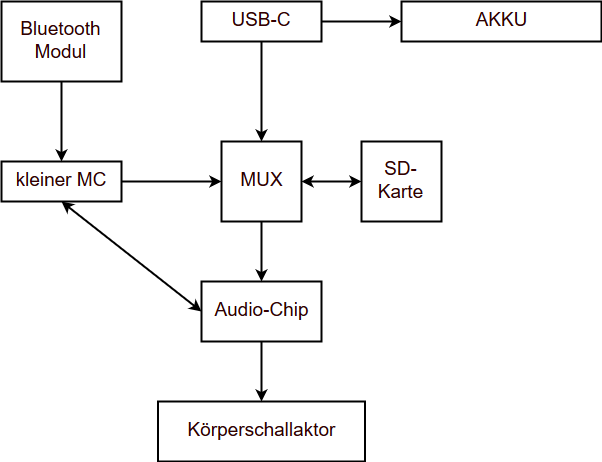
\includegraphics[width=120mm]{data/Loesungskonzept_alternativ.png}
	\caption{Alternatives Lösungskonzept} %picture caption
	\label{fig:first_layer}
\end{center}
\end{figure}



\section{Bluetooth}

\begin{figure}[H]
\begin{center}
	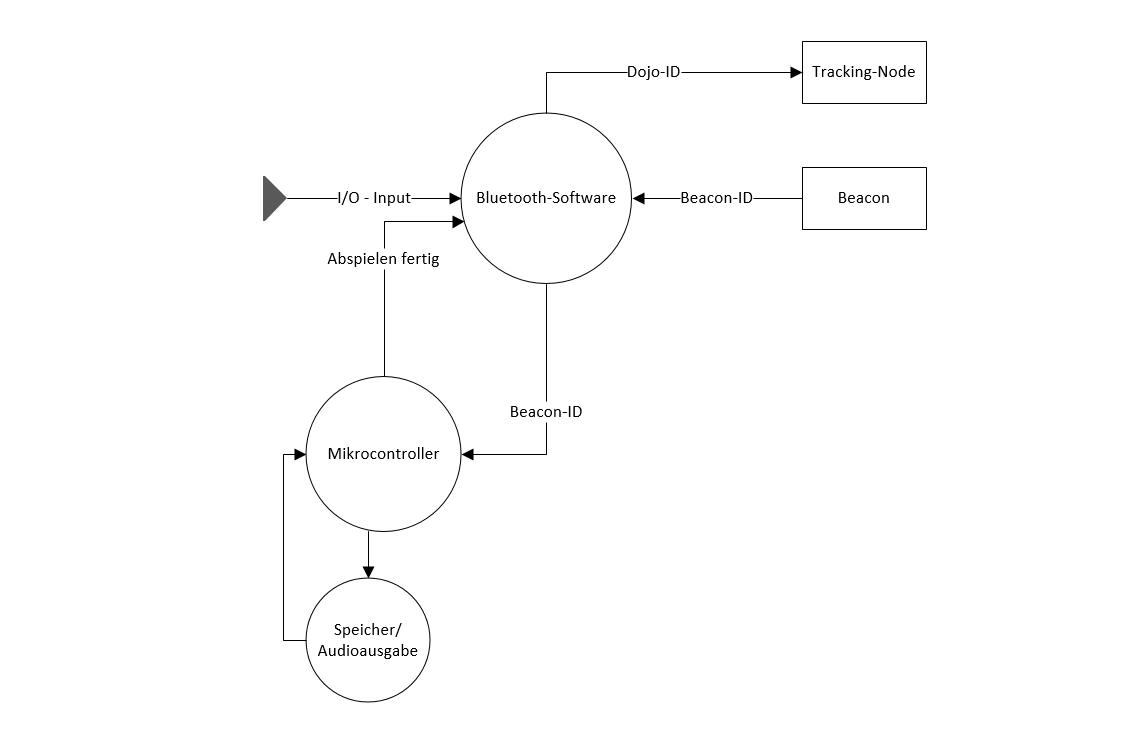
\includegraphics[width=120mm]{data/Bluetooth.png}
	\caption{Grobstruktur der Bluetooth-Software} %picture caption
	\label{fig:Grobstruktur_Bluetooth}
\end{center}
\end{figure}

Obenstehende Abbildung \ref*{fig:Grobstruktur_Bluetooth} zeigt die Grobstruktur der Bluetooth-Software. Über die Software erfolgt ein Input (Software – Input), welche das Suchen von Bluetooth Signalen in der Nähe auslöst. Vom Beacon mit dem stärksten Signal wird dann die Beacon-ID empfangen. Diese Beacon-ID wird Software-intern weitergeleitet, um das zugehörige Audio-File abzuspielen. Während des Abspielens der Audio-Datei ist das weitere Suchen deaktiviert, um Überschneidungen von Programmabläufen und daraus resultierende mögliche Fehler zu minimieren. Nach dem Abspielen einer Audio-Datei wird das Suchen wieder ermöglicht. Um den Raumzutritt zu kontrollieren, werden die Beacons in entsprechende Raumgruppen unterteilt, welche dann am Museumseingang von einem Mitarbeiter aktiviert oder deaktiviert werden können. Für ein mögliches Einbinden des Dojo in ein Tracking-System wird der Dojo in der Lage sein, seine eigene Erkennungsnummer auf Anfrage zu senden, ähnlich wie ein Beacon.
\subsection{Schnittstellen zu anderen Bereichen:}
Dojo soll, um Energie zu sparen, erst per Knopfdruck das Kunstobjekt mit der stärksten Signalstärke suchen und die entsprechende Datei dafür abspielen. Dies führt Software-intern zu einer Parameterübergabe an die Audio-/Speichersektion. Während der Audiowiedergabe soll das BT ausgeschaltet bleiben, weshalb wiederum Software-intern eine Parameterübergabe bzw. -Abfrage erfolgen muss. Dies soll verhindern, dass während der Audio-Wiedergabe das Suchen und Abspielen eines weiteren Objekts möglich ist. Beim Wunschziel Daten-Austausch herrscht eine enge Verbundenheit zwischen BT und Speicher. 

\section{Speichern und Audio}

Die Ausgabe der gewünschten Audio-Dateien wird mit einem sogenannten Körperschallaktor umgesetzt welcher in Abbildung \ref*{fig:schallaktorAdafruit} ersichtlich ist. Dieser ermöglicht es, die ausgesendeten Schwingungen über den Schädelknochen weiterzuleiten. Dadurch kann das Mittelohr umgangen werden und die Hygiene verbessert werden, da kein direkter Kontakt mit dem Gehörgang stattfindet. Für den Bau eines Prototyps wird ein Körperschallaktor des Herstellers Adafruit verwendet. 

\begin{figure}[H]
\begin{center}
	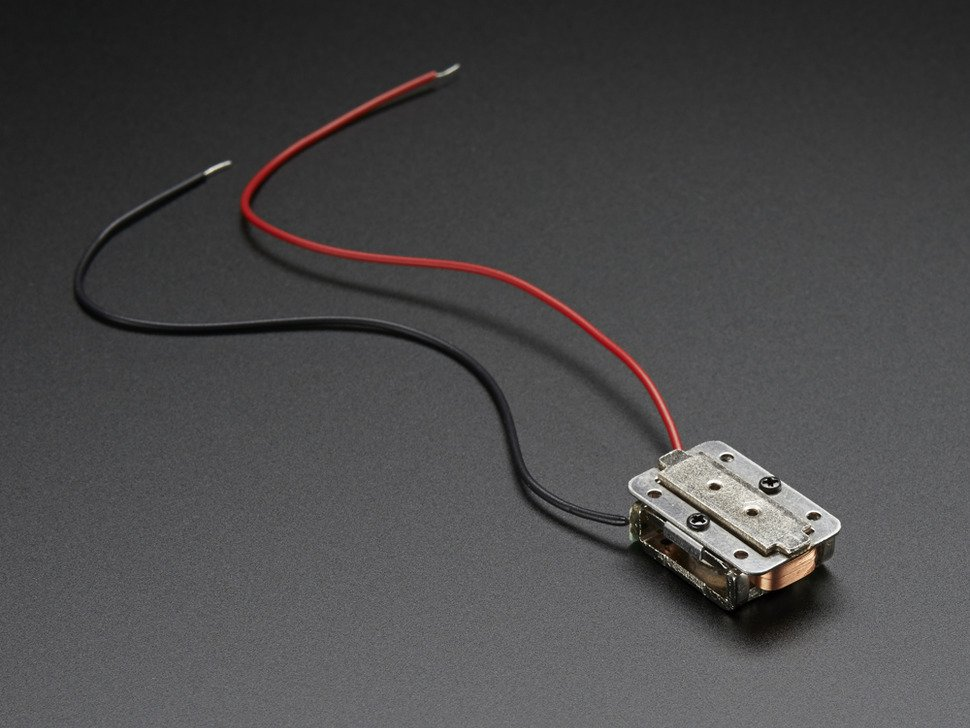
\includegraphics[width=110mm]{data/Schallaktor.png}
	\caption{Körperschallaktor von Adafruit}
	\label{fig:schallaktorAdafruit}
\end{center}
\end{figure}

Das Ziel ist es, bei möglichst geringem Energieverbrauch, eine möglichst intensive Lautstärke, bei guter Audioqualität zu erzielen.
Die Steuerung und Ausgabe der verschiedenen Audiosignale wird von einem zentralen Mikrocontroller übernommen. Ausserdem muss das Audiosignal verstärkt und bei Bedarf gefiltert werden. Damit der Energieverbrauch möglichst gering bleibt, wird die Verstärker und Filterstufe wenn möglich digital durch den Mikrocontroller umgesetzt. Dadurch kann die Anzahl der analogen Bauelemente verringert werden und somit auch der Platzbedarf klein gehalten werden.

Die Speichereinheit wird mit einer externen SD-Karte umgesetzt, die dann manuell entfernt und beschrieben werden kann. Das bedeutet auch, dass die Platzierung der SD-Karte möglichst elegant am Gehäuse erfolgen muss. Alternativ wird versucht den Datentransfer zur Aktualisierung der SD-Karte über die Bluetooth-Verbindung umzusetzen. Die Kommunikation über USB wird vernachlässigt. Damit der Mikrocontroller eine aktive Verbindung zur Speichereinheit hat, wird eine entsprechende Schnittstelle für den Datentransfer zwischen Speichereinheit und Mikrocontroller eingerichtet. Somit kann sich der Mikrocontroller entsprechend der Bluetooth-ID, das jeweils zugehörige Audio-File holen, über die Filter und Verstärkerstufe aufbereiten und anschliessend über den Körperschallaktor ausgeben.

\section{Energiespeicher}
\section{Induktives Laden}
Um den Energiespeicher des Dojos aufladen zu können, wird eine induktive Ladeschaltung eingebaut. In einer externen Ladevorrichtung wird die Netzspannung umgewandelt und auf eine Spule gegeben. Diese Spule erzeugt somit ein elektrisches Feld. Ist der Dojo in Reichweite zu dieser Apparatur und somit im induzierten Energiefeld, wird die Energie von diesem in elektromagnetischer Form in den Dojo transportiert und dort umgewandelt. In der Spule, die sich im Dojo befindet, wird so eine Wechselspannung induziert. Um diese Spannung für die Akkuladung nutzbar zu machen, wird diese mithilfe eines Gleichrichters angepasst und anschliessend noch geglättet. Die induktive Lademethode ermöglicht es, ein komplett geschlossenes Gehäuse zu verwenden. Dadurch ist der Dojo vor eindringender Feuchtigkeit oder Schmutz geschützt. Des Weiteren ist so seine Lebenszeit verlängert. Aufgrund fehlender Anschlüsse können auch keine Abnutzungserscheinungen auftreten, welche durch häufiges ein- und ausstecken auftreten können. 

\begin{figure}[H]
\begin{center}
	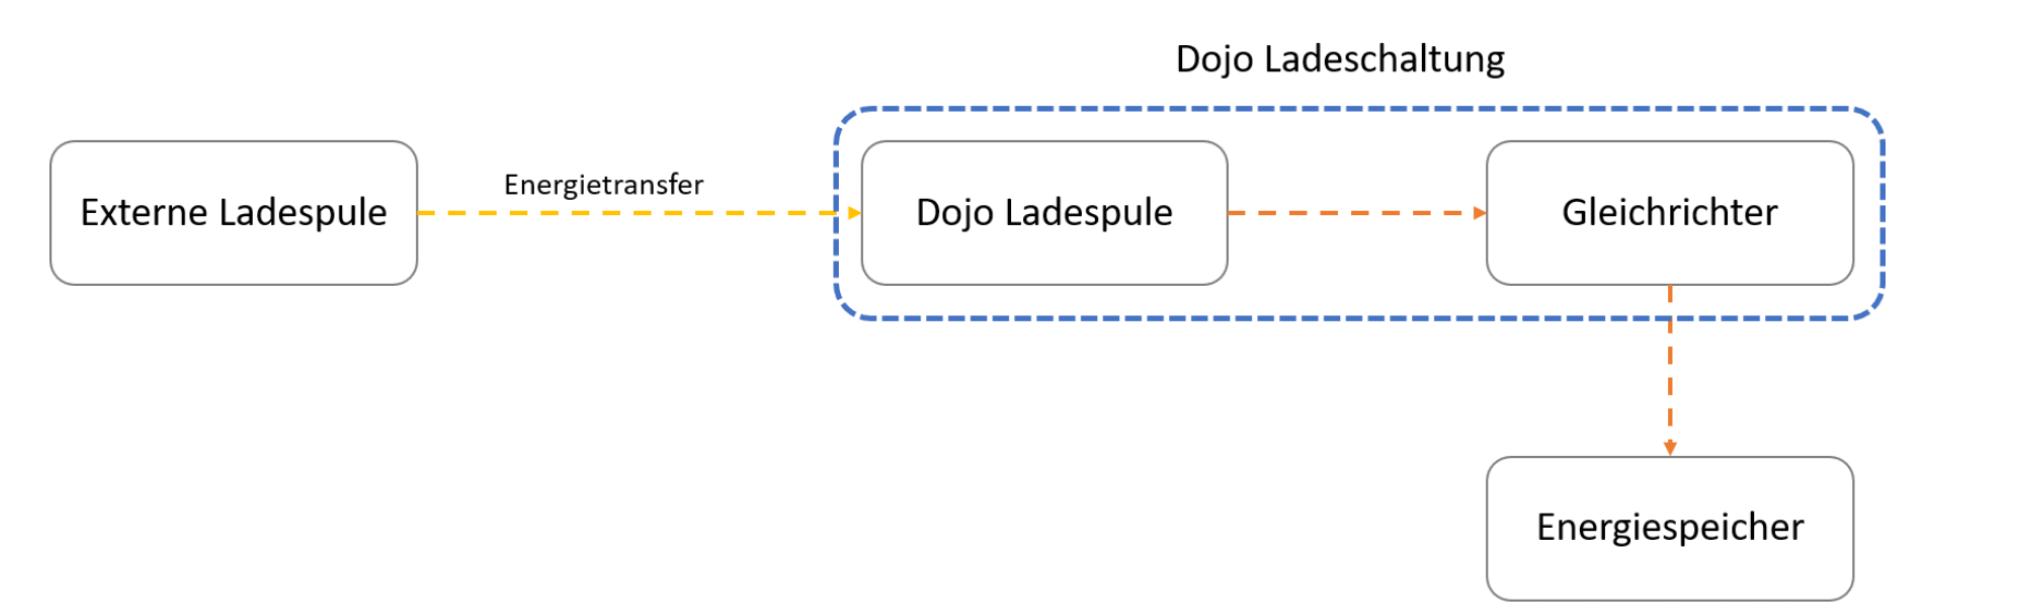
\includegraphics[width=160mm]{data/Induktion.png}
	\caption{Grobstruktur der Bluetooth-Software} %picture caption
	\label{fig:first_layer}
\end{center}
\end{figure}
\section{Testkonzept}
In den nachfolgenden Abschnitten wird erläutert, welche Teilsysteme und Komponenten getestet werden.

\subsection{Gesamtsystem}
Die ID eines Bluetooth-Beacons soll empfangen und entsprechend intepretiert werden. Aufgrund dieser ID wird dann das entprechende Audio-Signal vom Mikrocontroller aus dem Speicher geholt und abgespielt. 

\subsection{Audiowiedergabe}
Die Audiowiedergabe kann einzeln getestet werden. Dazu wird mit einem kleinen Testprogramm eine Audiodatei über den NRF52832 auf den Knochenschallaktor ausgegeben. Dabei kann die Audioausgabe auf die Funktionalität (Wird das Audio-File wiedergeben?) und die Qualität (Lautstärke, Verzerrung) getestet werden.

\subsection{Akkulaufzeit}
Um die Akkulaufzeit zu testen, wird mit dem Prototyp dauerhaft eine Audiodatei abgespielt. Dies verbraucht am meisten Energie und eignet sich somit bestens, um die maximale Laufzeit zu ermitteln. Für die Umsetzung wird dazu ein entsprechendes Testprogramm auf den Mikrocontroller geladen und ausgeführt.

\subsection{Tiefentladungsschutz}
Um die Funktion des Tiefentladungsschutz zu testen, wird der Akku bis auf seine untere Entladungsgrenze belastet und dann getestet ob der Tiefentladungsschutz das Gerät abschaltet. Dazu lassen sich zuvor berechnete Werte bestens mit gemessenen Werten vergleichen, um eine entsprechende Aussage über die Funktionalität machen zu können.

\subsection{Bluetooth}
Es wird überprüft ob ein Bluetooth Beacon erkannt werden kann und auf welche Entfernung er erkannt wird. Weiter wird das Systemverhalten bei mehreren vorhandenen ID-Signalen überprüft. Über die ID-Nummer oder über das auszugebende Audio-File kann erkannt werden, ob die richtige ID vom Mikrocontroller verarbeitet wird.

%%%%%%%%%%%%%%%%%%%%%%%%%%%%%%%%%%%%%%%%%%%%%%%%%%%%%%%%


\end{document}

